\chapter {Detailed Research Program}

In previous work Ariel's deep learning lab developed a multi-modal, deep-learning based architecture for detecting whether a command given to an autonomous assistant agent is a correction of a previous command \cite{nivasch2019correction}.  We show that using both vocal cues and text results at an increase in accuracy (when compared to using text or voice only). We believe that the same properties that hold in correction detection are true also for deception detection, and therefore intend to use  similar methods for deception detection.

\section{Goals}
The goal of this project is to build well performed autonomous agents which can work in a deception environment. Sub-goals to achieve this includes multi-model (speech and text) input analysis, user dynamics analysis (behavior and demographic statistics), deception dataset and labels collection, detection model development and human-computer interaction.

\subsection{Work Plan}
In the first phase of the work will focus on detecting deception in the ``cheat game'' environment.
The ``cheat game'' (also known as B.S. and the bluff game) is a turn taking card game where the players' goal is to get rid of all of their cards. After dealing 15 cards to each player, the game begins with a card flipped over from the deck of cards to a pile of cards.
On each turn a player may place up-to 4 cards on the pile of cards, these cards may either contain cards that are one higher than the current card or one lower. The cards placed on the pile are faced-down, so the player may claim to put cards that are different than what he actually put. If a player suspects that a different player is cheating, the player may call out a cheat, and then, if the player did actually cheat, he collects all the cards, otherwise, the player that called out a cheat collects the cards. Instead of placing cards on the pile, a player may draw 3 cards from the deck. In our local simulation process we found that a 2 player game might take too long.To prevent paid players to loose interest and leave mid game we limited each game to 12 minutes. This will result in a dataset that is not only labeled by whether each player is deceptive or not as a whole, but each statement will include whether the other opponent thought it was deceptive. The players will be paid using Amazon's Mechanical Turk service. Which allows researchers and hi-tech companies to collect and label data by hiring people from all over the world. due to language limitations and different accents we will limit our player to be from the US only.    

As to the fundamental module of the deception detection agent, i.e., the detection model, several issues will be studied in this project. First, we will explore the current classification models and their performance, then move a step forward to propose new models to detect deception with degree by leveraging data with scaling, or at least, the information that which is more possible to be a lie. Second, the factor of individuality in deception detection will be studied. Third, we plan to develop a model which can facilitate the received behavior related cues from autonomous agents and feedback its detection results to the agents to create a better communication environment. 

In the second phase we will built our deception detection model based on deep learning methods. The model will firstly preprocess the data. We will need to cut the beginning and the end of each recording using sound detector. After that we will turn the recordings into spectrogram images. The spectrograms have shown promising results in previous speech based modules. Once the preprocessing stage is done we will insert the image into our deep network. The sane default attempt will be using RNN or CRNN. The model will firstly label the sound samples binary simply stating whether a statement is true or false. Next we will build a ranking system to determine the amount of surety the model have to each claim. 

In the third phase we will build an autonomous agent to detect deception in real time. After training the model from phase II we will integrate it in a real time software connecting to the Cheat Game from phase I. The agent will play against real humans. We are hoping to show it will outplay them. Since, in order to complete a full game, the agent will also need to speak. We will set him only as a deception detection assistant. Meaning a real human will need to state the claims bu himself but calling a cheat and challenging the opponents claim will be done automatically using our agent.  


\section {Theoretical Results}


\section {Simulation Results}

We have developed an online version of the ``cheat game''.  We developed our game for two players, which we will call Alice and Bob. 
Alice selects the cards she wishes to dismiss, clicks a button and states her claim in speech (e.g. ``two sixes''). Alice must then click on the cards presenting her claim. We note that the current version involves no speech recognition. The claim is then played back to Bob who is required  to determine what he heard. Bob then places his cards, records his statement and so on. In case that Bob hears a statement different than what Alice claims her statement was, Alice collects all the cards. Alice may also open a dispute and the incident will be manually checked.

The ``cheat game'' provides us with a controlled domain in which users may either lie or tell the truth; the game provides us quality labels as well. We intend to deploy the game in a crowd-based platform (e.g. Mechanical Turk) and collect approximately 10,000 recordings. We will use the data to develop a good classifier that, given an utterance, will determine whether the statement is true or false. We will also develop a classifier that will predict whether a statement raises suspicion or not.
We will use these models to develop an agent that will play the ``cheat game'' with an attempt to outperform humans at this game

See Figure \ref{fig:cheatgamegui} for a screen-shot of the game.

\begin{figure}[tbph]
	\centering
	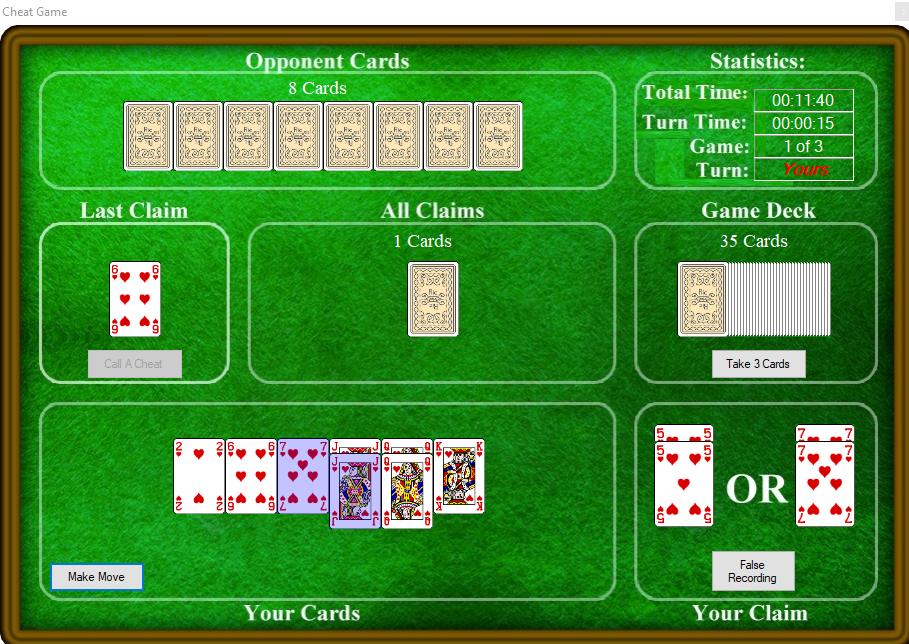
\includegraphics[width=4.5in]{Chapters/cheat_game_GUI}
	\caption{The graphical interfaced developed for the ``cheat game''.}
	\label{fig:cheatgamegui}
\end{figure}


Model wise, we have conducted experiments on students live play dataset, which includes 243 samples recorded in our lab by the students themselves as a study project. As a preliminary test, they encoded the dialogues with the RNN model and constructed a simple classifier to distinguish the deception from the truth. The results are shown in Tables ~\ref{Table:undergradsres} ~\ref{Table:undergradsres_pref}. Interestingly, we see that even on a small scale of data and with limited calculation resources it is possible to achieve a much better than random results. Meaning in our research, using a much larger and less heterogeneous dataset we believe we can transcend this results.   


\begin{table}[tbph]
	\centering
	\begin{tabular}{|c|c|l|}
		\hline
		\textbf{}              & \textbf{Correct prediction} & \textbf{False prediction} \\ \hline
		\textbf{True statment} & 100                         & 22                        \\ \hline
		\textbf{Lie statment}  & 66                          & 55                        \\ \hline
	\end{tabular}
	\caption{Lie detection results }
	\label{Table:undergradsres}
\end{table}

\begin{table}[tbph]
	\centering
	\begin{tabular}{|c|c|l|}
		\hline
		 \multicolumn{1}{|l|}{recall}    & \multicolumn{1}{l|}{precision}  & \multicolumn{1}{l|}{accuracy}  \\ \hline
		 \multicolumn{1}{|l|}{0.54} 		& \multicolumn{1}{l|}{0.75} & \multicolumn{1}{l|}{0.68} \\ \hline
                                                            
	\end{tabular}
	\caption{Lie detection performance on face too face game dataset. By undergrad students}
	\label{Table:undergradsres_pref}
\end{table}



